\chapter{Classical Mechanics and the Meaning of State}

Classical mechanics is introduced here not as one subject among many, but as the framework in which the general logic of physical evolution first becomes visible. These notes follow Leonard Susskind's opening lecture closely, using the transcript as the primary source and retaining a small amount of board evidence curated for this chapter by LazyingArt LLC and Video2Book where the layout of the argument matters. The lecture begins in a deliberately artificial world of discrete time and very simple systems, because that is the cleanest place to ask the first real question: what information must a system carry in order for the laws of physics to tell us what happens next?

\section{Opening Motivation and the Stroboscopic Toy World}

The lecture begins with a large claim: the basic framework of all physics is classical mechanics. That claim is then narrowed at once into a method. Instead of starting with planets, pendulums, or particles moving under realistic forces, we strip the subject to its bare bones and ask what a law of evolution even means.

The first simplification is temporal. Time will not flow continuously. We look at the world only at equally spaced beats of a stroboscopic light. If we label the beats by \(n=0,1,2,\ldots\), then the entire law of motion becomes an update rule from one beat to the next:
\begin{equation}
q_n \mapsto q_{n+1}.
\end{equation}
Here \(q_n\) is the state of the system at the \(n\)-th beat.

The second simplification is kinematical. We imagine systems so primitive that they have only a handful of possible configurations. The point of this move is not realism. The point is to isolate the structure of lawful evolution from the complications of geometry and force.

\section{Two States, One Law, and the Meaning of Phase Space}

The simplest nontrivial example is a coin laid on a table. It has two configurations: heads and tails. Let us denote the space of possibilities by
\begin{equation}
\Gamma=\{H,T\}.
\end{equation}

\begin{definition}
The phase space of a system is the space of its possible states.
\end{definition}

\begin{definition}
A state is a complete specification of the information needed to determine what happens next.
\end{definition}

At this stage phase space is as small as it could be while still allowing something to happen: two points in an abstract space, one labelled \(H\), the other \(T\). The lecture is careful here. Phase space is not yet a geometric arena like ordinary space. It is simply the set of possible states.

\subsection{Question \& Answer}

Question: What exactly counts as a state?

Answer: A state is not merely any description of the system. It is exactly enough information to determine the next step of the evolution. If a single label such as \(H\) or \(T\) is enough, then that is the state. If the law needs more information, then the state must be enlarged. This operational definition is the thread that runs through the whole lecture.

There is a useful contrast already lurking in the background. A world with only one state would be completely trivial: the only possible law would be that the system stays where it is forever. With two states, however, there is already room for distinct laws of nature.

\section{Arrow Diagrams and the First Deterministic Laws}

The next move is to turn the law itself into geometry. We represent each state by a point, and we represent the update rule by an arrow from the present state to the next state. The arrow is not decoration; it is the law.

The first law is the dull one:
\begin{equation}
H \mapsto H,\qquad T \mapsto T.
\end{equation}
If the coin is heads now, it will be heads at the next beat; if it is tails now, it will remain tails.

The second law is slightly more interesting:
\begin{equation}
H \mapsto T,\qquad T \mapsto H.
\end{equation}
Now the coin alternates forever:
\begin{equation}
H \mapsto T \mapsto H \mapsto T \mapsto \cdots
\end{equation}

\begin{figure}[htbp]
\centering

\includegraphics[width=0.72\textwidth]{lecture_01_figure_03.png}
\caption{Board evidence for the two-state coin system. On the left are the self-loops of the ``stay the same'' law; on the right the alternating law is being drawn.}
\end{figure}

\begin{figure}[htbp]
\centering
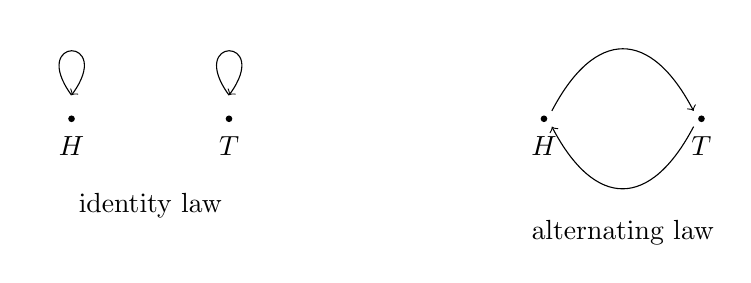
\begin{tikzpicture}[scale=1.0]
\fill (-4,0) circle (1.2pt);
\node at (-4,-0.35) {$H$};
\draw[->] (-4,0.30) .. controls (-4.55,1.05) and (-3.45,1.05) .. (-4,0.30);

\fill (-2,0) circle (1.2pt);
\node at (-2,-0.35) {$T$};
\draw[->] (-2,0.30) .. controls (-2.55,1.05) and (-1.45,1.05) .. (-2,0.30);

\node at (-3,-1.10) {identity law};

\fill (2,0) circle (1.2pt);
\node at (2,-0.35) {$H$};

\fill (4,0) circle (1.2pt);
\node at (4,-0.35) {$T$};

\draw[->] (2.10,0.10) .. controls (2.65,1.15) and (3.35,1.15) .. (3.90,0.10);
\draw[->] (3.90,-0.10) .. controls (3.35,-1.15) and (2.65,-1.15) .. (2.10,-0.10);

\node at (3,-1.45) {alternating law};
\end{tikzpicture}
\caption{A clean redraw of the two elementary laws on the two-state phase space. The reverse arrow in the alternating law is supplied by the transcript, not by the partially occluded frame alone.}
\end{figure}

These examples establish the language of the lecture. To know the future, one follows arrows. In these toy systems classical mechanics already looks like a collection of states equipped with a rule telling us where to go next.

\section{Allowed and Forbidden Laws in Finite State Spaces}

Once the arrow language is in place, the lecture stops cataloguing cute examples and asks the real question: which arrow diagrams are actually allowed by classical physics?

The first extension is from two states to six. A die has six states, and one possible law is the six-cycle
\begin{equation}
1\mapsto2,\qquad
2\mapsto3,\qquad
3\mapsto4,\qquad
4\mapsto5,\qquad
5\mapsto6,\qquad
6\mapsto1.
\end{equation}
This is already enough to show an important point: on a finite state space, an allowed law simply cycles through the states in some definite order.

The lecture also considers disconnected cycles, for example
\begin{equation}
1\mapsto1,\qquad
2\mapsto3,\qquad
3\mapsto4,\qquad
4\mapsto2,\qquad
5\mapsto6,\qquad
6\mapsto5.
\end{equation}
Here there is not one orbit but several. The system may remain fixed, or circulate in a three-cycle, or alternate in a two-cycle, depending on where it started.

Now come the forbidden laws. A typical bad example is
\[
1\mapsto2,\qquad 2\mapsto3,\qquad 3\mapsto2.
\]
This law is deterministic into the future: from each state there is a unique next step. But it is not deterministic into the past. If we find ourselves at state \(2\), we cannot tell whether we came from \(1\) or from \(3\).

Reversing all the arrows produces the opposite failure: the past is unique, but the future is not.

\begin{figure}[htbp]
\centering
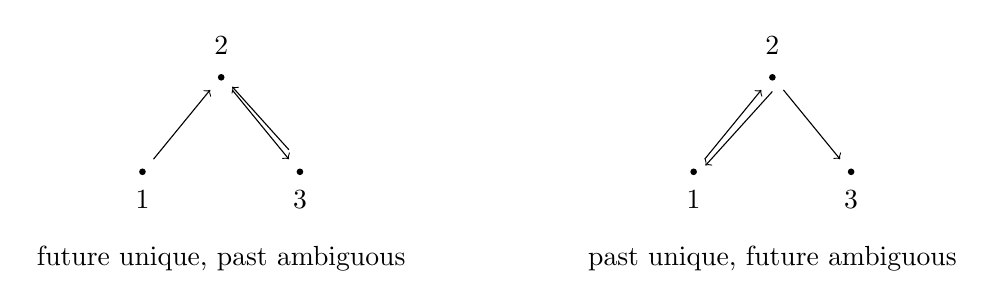
\begin{tikzpicture}[scale=1.0]
\fill (-5,0) circle (1.2pt);
\node at (-5,-0.35) {$1$};
\fill (-4,1.2) circle (1.2pt);
\node at (-4,1.60) {$2$};
\fill (-3,0) circle (1.2pt);
\node at (-3,-0.35) {$3$};

\draw[->] (-4.86,0.16) -- (-4.14,1.04);
\draw[->] (-3.86,1.04) -- (-3.14,0.16);
\draw[->] (-3.14,0.28) -- (-3.86,1.08);

\node at (-4,-1.10) {future unique, past ambiguous};

\fill (2,0) circle (1.2pt);
\node at (2,-0.35) {$1$};
\fill (3,1.2) circle (1.2pt);
\node at (3,1.60) {$2$};
\fill (4,0) circle (1.2pt);
\node at (4,-0.35) {$3$};

\draw[->] (2.14,0.16) -- (2.86,1.04);
\draw[->] (3.14,1.04) -- (3.86,0.16);
\draw[->] (3.00,1.02) -- (2.15,0.08);

\node at (3,-1.10) {past unique, future ambiguous};
\end{tikzpicture}
\caption{Two forbidden three-state laws. The first loses the past; the second loses the future.}
\end{figure}

\begin{proposition}
For a finite phase space, an allowed classical law is a bijection of the state set. Equivalently, every state has exactly one incoming arrow and exactly one outgoing arrow.
\end{proposition}

\begin{proof}
If a state had two outgoing arrows, the future would not be unique. If it had no outgoing arrow, evolution would stop. If a state had two incoming arrows, the past would not be unique. If it had no incoming arrow, the law could not be run backward through that state. Thus classical evolution on a finite state space requires one in-arrow and one out-arrow at every point. On a finite set that is exactly the condition for a bijection.
\end{proof}

\begin{remark}
This is the discrete skeleton of reversibility. A finite classical law is not just deterministic forward in time. It preserves enough information that the past is also uniquely recoverable.
\end{remark}

\subsection{Question \& Answer}

Question: Why must an allowed classical law have one arrow in and one arrow out at every state?

Answer: Because classical mechanics, as presented here, is deterministic in both directions. One outgoing arrow gives a unique future. One incoming arrow gives a unique past. If either uniqueness fails, information about the trajectory is lost, and the law is no longer acceptable as a classical law.

\section{Infinite State Spaces, Conservation, and Information}

The lecture then relaxes the assumption that phase space must be finite. We may instead imagine an infinite line of states labelled by integers
\[
\ldots,-2,-1,0,1,2,\ldots
\]
with the law
\begin{equation}
n \mapsto n+1.
\end{equation}
Every state still has one incoming arrow and one outgoing arrow. The difference is only that the trajectory no longer cycles through a finite set; it marches off forever.

This makes room for a new idea. Phase space can break into disconnected pieces. One piece may be an infinite chain, another a closed cycle, another a fixed point. The system never jumps from one component to another. That fact can be rephrased as a conservation law.

Suppose we assign the label \(C=+1\) to one connected component and \(C=-1\) to another. Then the motion preserves that label:
\begin{equation}
C_{n+1}=C_n.
\end{equation}
In this sense a conservation law is a memory of where the system started. The system retains some piece of information for all time.

This is why the lecture connects reversibility with information conservation. If we always know where the system came from and where it is going, then no information about its location in phase space has been lost. If two distinct histories merge into one present state, information has been destroyed.

The lecture puts this sharply: information conservation is perhaps the most fundamental structural law of classical physics. Why the laws of nature have this form is not derived here; it is presented as an experimental fact about the known laws.

\section{Continuous Motion and Why Position Alone Is Not Enough}

The real world, of course, is not a stroboscopic toy world with finitely many states. So the lecture now asks the continuous analogue of the earlier question. Suppose a particle moves along a line. Is its position enough to count as its state?

\subsection{Question \& Answer}

Question: Is knowing the position of a particle enough to know what happens next?

Answer: No. To know where the particle will be next, we must know not only where it is, but how fast it is moving and in which direction. Position alone does not determine the next step. Velocity must be included.

Thus the state of a particle on a line is not just \(x\). It is
\begin{equation}
\text{state}=(x,v),\qquad v=\dot{x}.
\end{equation}
The phase space is therefore two-dimensional. One axis records position, the other velocity. Positive velocity means motion to the right; negative velocity means motion to the left.

\begin{figure}[htbp]
\centering

\includegraphics[width=0.74\textwidth]{lecture_01_figure_05.png}
\caption{Board evidence for the local flow picture of deterministic evolution. The frame supports the sparse geometry of the sketch rather than a full formal phase-plane diagram.}
\end{figure}

\begin{figure}[htbp]
\centering
\begin{tikzpicture}[scale=1.0]
\draw (-4,0) -- (4,0);
\fill (3,0) circle (1.2pt);
\node at (3.25,-0.35) {$x$};

\draw[->] (-0.70,0.95) -- (-0.20,0.75);
\draw[->] (-0.15,1.05) -- (0.35,0.85);
\draw[->] (0.40,0.90) -- (0.85,0.72);
\end{tikzpicture}
\caption{A sparse redraw of the local flow sketch on the board. The lecture uses such arrows to mean: from this state, here is where you go next.}
\end{figure}

The lecture then makes the picture more explicit. If the particle has zero velocity, its next position is the same position. If it has positive velocity, its next position lies to the right. If the positive velocity is larger, the step to the right is larger. If the velocity is negative, the next position lies to the left.

\begin{figure}[htbp]
\centering
\begin{tikzpicture}[scale=0.95]
\draw[->] (-4.2,0) -- (4.4,0);
\node at (4.65,0) {$x$};
\draw[->] (0,-2.4) -- (0,2.5);
\node at (0.30,2.25) {$v$};

\fill (0,0) circle (1.2pt);
\draw[->] (0.18,0.12) .. controls (0.52,0.38) and (0.52,-0.38) .. (0.18,-0.12);

\fill (1.2,0.9) circle (1.2pt);
\draw[->] (1.35,0.9) -- (2.05,0.9);

\fill (-1.2,1.5) circle (1.2pt);
\draw[->] (-1.05,1.5) -- (0.10,1.5);

\fill (1.4,-0.9) circle (1.2pt);
\draw[->] (1.25,-0.9) -- (0.55,-0.9);

\fill (-1.3,-1.6) circle (1.2pt);
\draw[->] (-1.45,-1.6) -- (-2.70,-1.6);
\end{tikzpicture}
\caption{Transcript-backed phase space for motion on a line. Above the horizontal axis the arrows point to the right; below it they point to the left; on the axis itself the position does not change at the next instant.}
\end{figure}

The point is not merely pictorial. The very meaning of phase space has changed. In the toy coin model a point of phase space was just one of the labels \(H\) or \(T\). For a particle on a line, a point of phase space is a pair \((x,v)\). That is the smallest package of information that determines the next step.

\begin{remark}
The lecture pauses here over an important practical subtlety. Classical equations are deterministic in principle, but they are not infinitely predictable in practice, because the initial state is specified by real numbers and real numbers are never known with infinite precision. Errors may remain small for a long time, or they may grow rapidly in chaotic systems. Nevertheless, for any fixed time interval, classical mechanics says that sufficiently precise initial data would in principle determine the motion over that interval.
\end{remark}

\section{First-Order Versus Second-Order Equations, and the Return to Two-Step Memory}

The lecture now translates the phase-space lesson into the language of differential equations. If the state must contain both position and velocity, then the equations of motion should reflect that fact.

A first-order equation contains only first time derivatives; a second-order equation contains accelerations as well. The notation used throughout is the dot notation:
\[
\dot{x}=\frac{dx}{dt},\qquad \ddot{x}=\frac{d^2x}{dt^2}.
\]

To make the point as sharply as possible, the lecture first invents a phony law:
\begin{equation}
F(x)=m\dot{x}.
\end{equation}
Here the force depends only on position. If we know \(x\), then we know \(F(x)\), and therefore we know \(\dot{x}\). Position alone would determine the immediate motion. Differentiating once more,
\begin{align}
\frac{dF}{dt} &= m\ddot{x},\\
\frac{dF}{dt} &= \frac{dF}{dx}\frac{dx}{dt}=\frac{dF}{dx}\,\dot{x}.
\end{align}
So once \(x\) is known, \(\dot{x}\) is known from the fake equation, and then \(\ddot{x}\) is known as well. Repeating the process would determine higher derivatives too. A first-order law of this sort would therefore require only one state variable.

But Newton's equation is not this equation. Newton's equation is
\begin{equation}
F(x)=m\ddot{x}.
\end{equation}
If we know \(x\), then we know the force and hence the acceleration. But there is still no equation that tells us the velocity. Therefore position alone is not enough. We must add \(\dot{x}\) as independent initial data. That is exactly why the phase space of a particle on a line is two-dimensional.

This is the same structural point we met in the toy models, now stated in the language of calculus. The order of the differential equation measures how much information a state must contain.

\subsection{Question \& Answer}

Question: What if the next state depends on the previous two configurations?

Answer: Then a single symbol \(H\) or \(T\) is not a state. The state must be enlarged so that it includes the previous two entries. In other words, the law may still be deterministic and reversible, but only on a larger phase space.

The lecture returns to the coin precisely to make this point concrete. If the update rule depends on the last two outcomes, then the appropriate phase space is
\begin{equation}
\Gamma_2=\{HH,HT,TH,TT\}.
\end{equation}
A clean reversible completion of the classroom discussion is, for example,
\begin{equation}
HH\mapsto HH,\qquad
HT\mapsto TT,\qquad
TT\mapsto TH,\qquad
TH\mapsto HT.
\end{equation}
This is now a deterministic reversible law on four states. The difficulty was never that the law was impossible. The difficulty was that the original state space \(\{H,T\}\) was too small.

Once that lesson is understood, the higher-order generalization is immediate. If classical mechanics had required positions, velocities, and accelerations as independent data, then the equations of motion would have been third order in time and phase space would have had to include
\[
(x,\dot{x},\ddot{x}).
\]
The lecture emphasizes that this is not what experiment tells us. Classical mechanics stops at positions and velocities. Already a single particle in ordinary three-dimensional space therefore has six phase-space coordinates: three positions and three velocities.

\section{Summary}

The lecture begins with the claim that classical mechanics provides the structural template for physics, and it spends the rest of the hour making that claim precise. We first learn to think in terms of phase space, then to define a state as whatever information is needed to determine the next step, then to recognize classical evolution as a deterministic and reversible flow on that phase space. In finite systems this becomes the rule of one in-arrow and one out-arrow; in continuous systems it becomes the statement that a particle on a line is described by \((x,v)\), not by \(x\) alone.

The last step closes the circle. The order of the equations of motion is not an algebraic accident. It is a statement about how much information the world carries from one instant to the next. In that sense, the lecture's central theme is already fully visible in the first meeting: classical mechanics is the study of lawful evolution as conservation of information.